\pagenumbering{arabic}
\section{异常检查}
支持向量机(Support Vector Machies)是由Vapnik等人于1995年提出来的。之后随着统计理论的发展,支持向量机也逐渐受到了各领域研究者的关注,在很短的时间就得到很广泛的应用。支持向量机是建立在统计学习理论的VC维理论和结构风险最小化原理基础上的,利用有限的样本所提供的信息对模型的复杂性和学习能力两者进行了寻求最佳的折衷,以获得最好的泛化能力。SVM的基本思想是把训练数据非线性的映射到一个更高维的特征空间(Hilbert空间)中,在这个高维的特征空间中寻找到一个超平面使得正例和反例两者间的隔离边缘被最大化。SVM的出现有效的解决了传统的神经网络结果选择问题、局部极小值、过拟合等问题。并且在小样本、非线性、数据高维等机器学习问题中表现出很多令人注目的性质,被广泛地应用在模式识别,数据挖掘等领域(张学工 2000;崔伟东2001)。支持向量机可以用于分类和回归问题,本章着重介绍分类相关的知识。\\

\subsection{离群点检测}


就餐饮企业而言,经常会碰到这样的问题:

\begin{itemize}[leftmargin=1cm]

\item 如何根据客户的消费记录检测是否为异常刷卡消费?

\item 如何检测是否有异常订单?

\end{itemize}

这一类异常问题可以通过离群点检测解决。

离群点检测是数据挖掘中重要的一部分,它的任务是发现与大部分其他对象显著不同的对象。大部分数据挖掘方法都将这种差异信息视为噪声而丢弃,然而在一些应用中,罕见的数据可能蕴含着更大的研究价值。

在数据的散布图中,如图2-1离群点远离其它数据点。因为离群点的属性值明显偏离期望的或常见的属性值,所以离群点检测也称偏差检测。

\begin{figure}[thbp!]
\centering
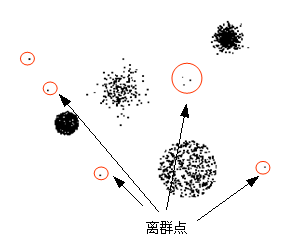
\includegraphics[width=0.4\linewidth]{figure/2-1}
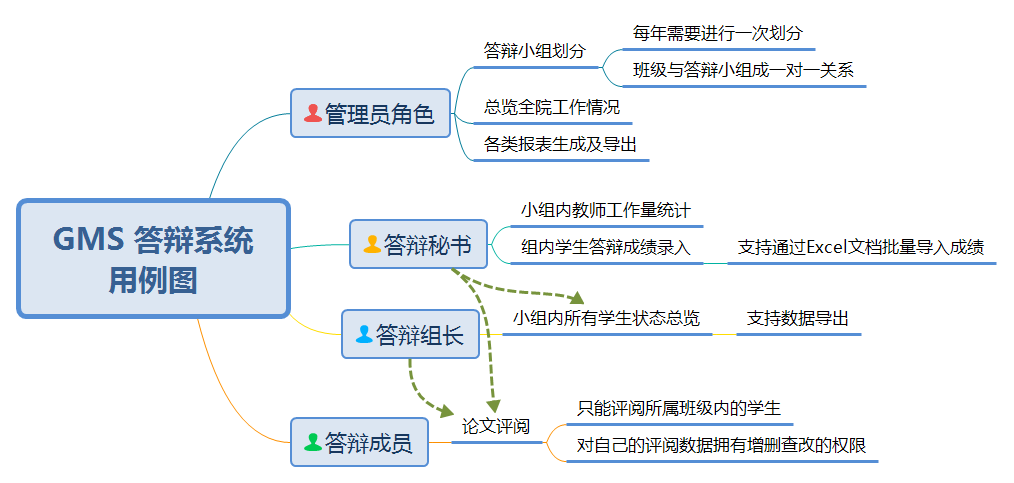
\includegraphics[width=0.4\linewidth]{figure/2-2}
\caption{\ 离群点检测示意图}
\label{fig:2-2}
\end{figure}

%latex自动控制页面布局,一般你不需要管页面
离群点检测已经被广泛应用于电信和信用卡的诈骗检测、贷款审批、电子商务中、网络入侵、天气预报等领域,如可以利用离群点检测分析运动员的统计数据,以发现异常的运动员。

\begin{itemize}[leftmargin=1cm]

\item 离群点的成因 离群点的主要成因有:数据来源于不同的类、自然变异、数据测量和收集误差。

\item 离群点的类型  对离群点的大致分类见表2-1
\end{itemize}

\begin{table}[thbp]\footnotesize
\caption{离群点的大致分类}
\begin{center}
\begin{tabular}{c|cl}
\hline  分类标准& 分类名称 & 分类描述  \\ 
\hline 从数据范围 & 全局离群点和局部离群点 & 从整体来看,某些对象没有离群特征, \\ 
& & 但是从局部来看,却显示了一定的离群性。\\ 
& & 如图2-2:C是全局离群点,D是局部离群点。 \\ 
\hline 从数据类型 & 数值型离群点和分类型离群点 & 这是以数据集的属性类型进行划分的。  \\ 
\hline 属性的个数 & 一维离群点和多维离群点 & 一个对象可能有一个或多个属性。 \\ 
\hline
\end{tabular} 
\end{center}
\label{tb:filter}
\end{table}

\begin{figure}[thbp!]
\centering
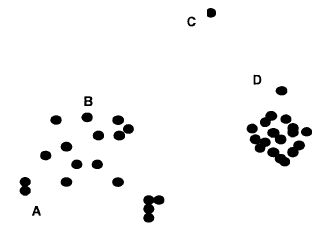
\includegraphics[width=0.4\linewidth]{figure/2-3}
\caption{\ 全局离群点和局部离群点}
\label{fig:2-3}
\end{figure}

%\end{enumerate}


\subsubsection{离群点检测方法}

常用离群点检测方法见表\ref{tb:filter1}

\begin{table}[thbp]%表格你自己再调整,很简单,就是再插入行,然后不加hline,一列不放数据
\footnotesize
\caption{常用离群点检测方法}
\begin{center}
\begin{tabular}{|l|l|l|}
\hline  离群点检测方法& 方法描述 & 方法评估  \\ 
\hline 基于统计 & 大部分的基于统计的离群点检& 基于统计模型的离群点检测方法 \\  
&测方法是构建一个概率分布模型, &的前提是必须知道数据集服从什么分布; \\
&并计算对象符合该模型的概率,&对于高维数据,检验效果可能很差。\\
&把具有低概率的对象视为离群点。& \\
\hline 基于邻近度 & 通常可以在数据对象之间定义邻近性度量, & 简单,二维或三维的数据可以做散点图观察;  \\ 
& 把远离大部分点的对象视为离群点。&大数据集不适用;对参数选择敏感;具有全局\\
& & 阈值,不能处理具有不同密度区域的数据集。\\
\hline 基于密度 & 考虑数据集可能存在不同密度区域这一事实, & 给出了对象是离群点的定量度量, \\ 
&从基于密度的观点分析,离群点是在低密度区域中的对象。&并且即使数据具有不同的区域也能够很好的处理;\\
&一个对象的离群点得分是该对象周围密度的逆。&大数据集不适用;参数选择是困难的。\\
\hline 基于聚类 & 一种是利用聚类检测离群点的方法是丢弃远离其他簇的小簇;& 基于聚类技术来发现离群点可能是高度有效的; \\ 
&另一种更系统的方法,首先聚类所有对象,&聚类算法产生的簇的质量对该算法产生\\
&然后评估对象属于簇的程度(离群点得分)。 &的离群点的质量影响非常大。\\
\hline

\end{tabular} 
\end{center}
\label{tb:filter1}%label 是唯一的
\end{table}

基于统计模型的离群点检测方法需要满足统计学原理,如果分布已知,则检验可能非常有效。基于邻近度的离群点检测方法比统计学方法更一般、更容易使用,因为确定数据集有意义的邻近度量比确定它的统计分布更容易。基于密度的离群点检测与基于邻近度的离群点检测密切相关,因为密度常用邻近度定义:一种是定义密度为到K个最邻近的平均距离的倒数,如果该距离小,则密度高;另一种是使用DBSCAN聚类算法,一个对象周围的密度等于该对象指定距离d内对象的个数。

本节重点介绍基于统计模型和聚类的离群点检测方法。
\subsubsection{基于模型的离群点检测方法}
通过估计概率分布的参数来建立一个数据模型,如果一个数据对象不能很好地跟该模型拟合,即如果它很可能不服从该分布,则它是一个离群点。

%大段落不能用itemize
%\begin{itemize}[leftmargin=1cm]

(1) 一元正态分布中的的离群点检测

正态分布是统计学中最常用的分布之一。

若随机变量$x$的密度函数$\varphi(x)=\frac{1}{\sqrt{2\pi}}e\frac{-(x-\mu)^2}{2\sigma^2}(x\in R)$,则称$x$服从正态分布,简称$x$服从正态分布$N(\mu,\sigma)$,其中参数$\mu$和$\sigma$分别为均值和标准差。

图2-3显示$N(0,1)$的密度函数:
\begin{figure}[thbp!]
\centering
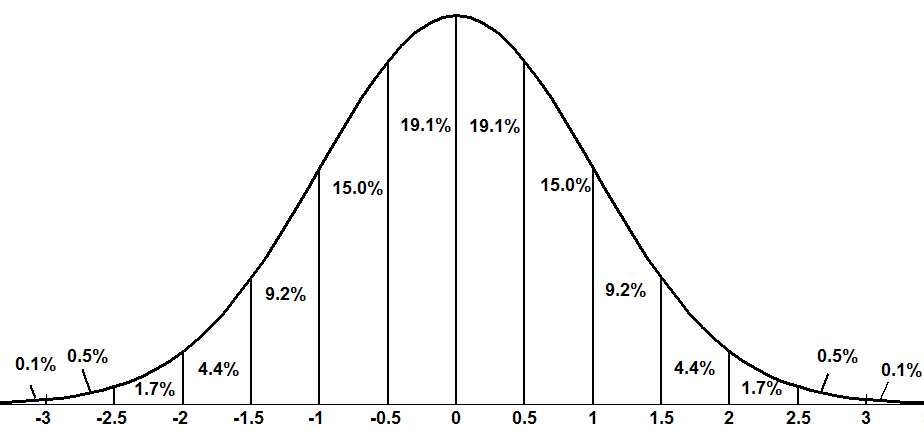
\includegraphics[width=0.4\linewidth]{figure/2-6}
\caption{$N(0,1)$的概率密度函数}
\label{fig:2-6}
\end{figure}

$N(0,1)$的数据对象出现在该分布的两边尾部的机会很小,因此可以用它作为检测数据对象是否是离群点的基础。数据对象落在三倍标准差中心区域之外的概率仅有0.0027。

(2)混合模型的离群点检测

这里首先介绍下混合模型。混合是一种特殊的统计模型,它使用若干统计分布对数据建模。每一个分布对应一个簇,而每个分布的参数提供对应簇的描述,通常用中心和发散描述。

混合模型将数据看作从不同的概率分布得到的观测值的集合。概率分布可以是任何分布,但是通常是多元正态的,因为这种类型的分布不难理解,容易从数学上进行处理,并且已经证明在许多情况下都能产生好的结果。这种类型的分布可以对椭圆簇建模。

总的讲,混合模型数据产生过程为:给定几个类型相同但参数不同的分布,随机地选取一个分布并由它产生一个对象。重复该过程次,其中是对象的个数。

具体地讲,假定有$K$个分布和$m$个对象$\chi=\{x_1,x_2,...,x_m\}$。设第$ j$个分布的参数为$\alpha_j$,并$A$设是所有参数的集合,即$A=\{\alpha_1,\alpha_2,...,\alpha_k\}$。则$p(x_i|a_j)$是第$i$个对象来自第$j$个分布的概率。选取第$j$个分布产生一个对象的概率由权值$w_j\{1\le j\le K\}$给定,其中权值(概率)受限于其和为1的约束,即$\sum_{j=1}^k w_j=1$。于是,对象$x$的概率由以下公式给出:
\begin{equation}p(x|A)=\sum_{j=1}^k w_jP_j(x|\theta_j)\end{equation}
如果对象以独立的方式产生,则整个对象集的概率是每个个体对象$x_i$的概率的乘积,公式如下:
\begin{equation}p(\chi|\alpha)=\prod_{i=1}^m P(x_i|\alpha)=\prod_{i=1}^m\sum_{j=1}^k w_jP_j(x|\alpha_j)\end{equation}
对于混合模型,每个分布描述一个不同的组,即一个不同的簇。通过使用统计方法,可以由数据估计这些分布的参数,从而描述这些分布(簇)。也可以识别哪个对象属于哪个簇。然而,混合模型只是给出具体对象属于特定簇的概率。

聚类时,混合模型方法假定数据来自混合概率分布,并且每个簇可以用这些分布之一识别。同样,对于离群点检测,数据用两个分布的混合模型建模,一个分布为正常数据,而另一个为离群点。

聚类和离群点检测的目标都是估计分布的参数,以最大化数据的总似然。

这里提供一种离群点检测常用的简单的方法:先将所有数据对象放入正常数据集,这时离群点集为空集;再用一个迭代过程将数据对象从正常数据集转移到离群点集,只要该转移能提高数据的总似然。

具体操作如下:

假设数据集U包含来自两个概率分布的数据对象:M是大多数(正常)数据对象的分布,而N是离群点对象的分布。数据的总概率分布可以记作:

 $U(x)=(1-\lambda)M(x)+\lambda N(x)$其中,$x$是一个数据对象;$\lambda\in[0,1]$,给出离群点的期望比例。分布$M$由数据估计得到,而分布$N$通常取均匀分布。设$M_t$和$N_t$分别为时刻$t$正常数据和离群点对象的集合。初始$t=0$,$M_0=D$,而$N_0=\emptyset$。

根据混合模型中公式$p(x|A)=\sum_{j=1}^k w_jP_j(x|\theta_j)$推导,在整个数据集的似然和对数似然可分别由下面两式给出:
\begin{equation} 
L_t(U)=\prod_{x_i\in U } P_U(x_i)=\bigg ((1-\lambda)^{|M_t|} \prod_{x_i\in M_i} P_{M_i}(x_i) \bigg)\bigg(\lambda^{|N_t|} \prod_{x_i\in N_i}P_{N_i}(x_i)\bigg) 
\end{equation}
\begin{equation}
\ln L_t(U)=|M_t|\ln (1-\lambda)+\sum_{x_i \in M_i }\ln P_{M_i}(x_i)+|N_t|\ln \lambda +\sum_{x_i \in N_i }\ln P_{N_i}(x_i)
\end{equation}
其中$P_D$、$P_{M_t}$、$P_{N_t}$分别是$D$、$M_t$、$N_t$的概率分布函数。

因为正常数据对象的数量比离群点对象的数量大的很多,因此当一个数据对象移动到离群点集后,正常数据对象的分布变化不大。在这种情况下,每个正常数据对象的正常数据对象的总似然的贡献保持不变。此外,如果假定离群点服从均匀分布,则移动到离群点集的每一个数据对象对离群点的似然贡献一个固定的量。这样,当一个数据对象移动到离群点集时,数据总似然的改变粗略地等于该数据对象在均匀分布下的概率(用$1-\lambda$加权)减去该数据对象在正常数据点的分布下的概率(用加权)。从而,离群点由这样一些数据对象组成,这样数据对象在均匀分布下的概率比正常数据对象分布下的概率高。

在某些情况下是很难建立模型的。如:因为数据的统计分布未知或没有训练数据可用。在这种情况下,可以考虑另外其他不需要建立模型的检测方法。

\subsubsection{基于聚类的离群点检测方法}
聚类分析用于发现局部强相关的对象组,而异常检测用来发现不与其他对象强相关的对象。因此聚类分析非常自然地可以用于离群点检测。本节主要介绍两种基于聚类的离群点检测方法。



(1)丢弃远离其他簇的小簇

一种利用聚类检测离群点的方法是丢弃远离其他簇的小簇。通常,该过程可以简化为丢弃小于某个最小阈值的所有簇。

这个方法可以和其他任何聚类技术一起使用,但是需要最小簇大小和小簇与其他簇之间距离的阈值。而且这种方案对簇个数的选择高度敏感,使用这个方案很难将离群点得分附加到对象上。

图2-4中,聚类簇数K=2,可以直观地看出其中一个包含5个对象的小簇远离大部分对象,可以视为离群点。

\begin{figure}[thbp!]
\centering
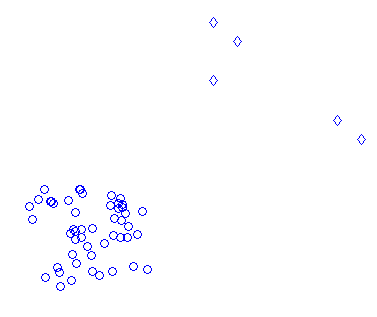
\includegraphics[width=0.4\linewidth]{figure/2-7}
\caption{\ K-Means算法的聚类图}
\label{fig:2-7}
\end{figure}

(2)基于原型的聚类

另一种更系统的方法,首先聚类所有对象,然后评估对象属于簇的程度(离群点得分)。在这种方法中,可以用对象到它的簇中心的距离来度量属于簇的程度。特别地,如果删除一个对象导致该目标的显著改进,则可将该对象视为离群点。例如,在K均值算法中,删除远离其相关簇中心的对象能够显著地改进该簇的误差平方和(SSE)。

对于基于原型的聚类,评估对象属于簇的程度(离群点得分)主要有两种方法:一是度量对象到簇原型的距离,并用它作为该对象的离群点得分;二是考虑到簇具有不同的密度,可以度量簇到原型的相对距离,相对距离是点到质心的距离与簇中所有点到质心的距离的中位数之比。

如图2-5,如果选择聚类簇数K=3,则对象A、B、C应分别属于距离它们最近的簇,但相对于簇内的其他对象,这三个点又分别远离各自的簇,所以有理由怀疑对象A、B、C是离群点。


\begin{figure}[thbp!]
\centering
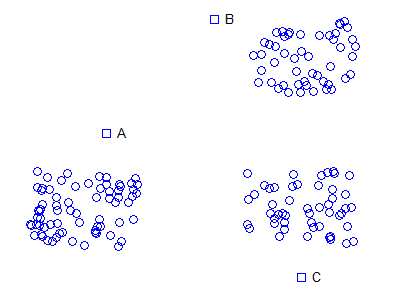
\includegraphics[width=0.4\linewidth]{figure/2-8}
\caption{\ 基于距离的离群点检测}
\label{fig:2-8}
\end{figure}


诊断步骤如下:


(1)进行聚类。

选择聚类算法(如K-Means算法),将样本集聚为K簇,并找到各簇的质心。

(2)计算各对象到它的最近质心的距离。

(3)计算各对象到它的最近质心的相对距离。

(4)与给定的阈值作比较。

如果某对象距离大于该阈值,就认为该对象是离群点。



基于聚类的离群点检测的改进:



(1)离群点对初始聚类的影响:通过聚类检测离群点时,离群点会影响聚类结果。为了处理该问题,可以使用如下方法:对象聚类,删除离群点,对象再次聚类(这个不能保证产生最优结果)。

(2)还有一种更复杂的方法:取一组不能很好的拟合任何簇的特殊对象,这组对象代表潜在的离群点。随着聚类过程的进展,簇在变化。不再强属于任何簇的对象被添加到潜在的离群点集合;而当前在该集合中的对象被测试,如果它现在强属于一个簇,就可以将它从潜在的离群点集合中移除。聚类过程结束时还留在该集合中的点被分类为离群点(这种方法也不能保证产生最优解,甚至不比前面的简单算法好,在使用相对距离计算离群点得分时,这个问题特别严重)。

对象是否被认为是离群点可能依赖于簇的个数(如k很大时的噪声簇)。该问题也没有简单的答案。一种策略是对于不同的簇个数重复该分析。另一种方法是找出大量小簇,其想法是:

\begin{itemize}[leftmargin=1cm]

\item 较小的簇倾向于更加凝聚;

\item 如果存在大量小簇时一个对象是离群点,则它多半是一个真正的离群点。

不利的一面是一组离群点可能形成小簇从而逃避检测。
\end{itemize}



“Detect Outlier(Distances)”基于距离的离群点检测,参数设置中可设定要检测的离群点的个数,如图2-6。

\begin{figure}[thbp!]
\centering
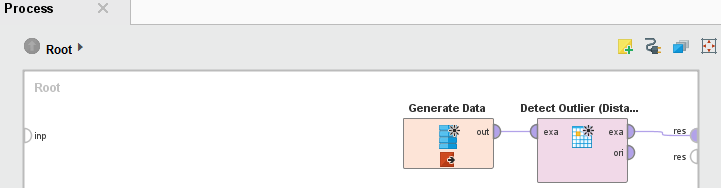
\includegraphics[width=0.4\linewidth]{figure/2-9}
\caption{\  RapidMiner自带的离群点检测流程}
\label{fig:2-9}
\end{figure}


第三方离群点检测插件带有功能更强的离群点检测功能,例如“One-Class LIBSVM Anomaly Score”为半监督的离群点检测操作符。

 离群点检测实例

下面,我们自己生成一个数据,来看看离群点检测的功能。

第一步:生成随机数据

调用“Generate Data”生成数据操作符,能帮助我们自动创建一些测试数据,创建参数设置图2-7。

\begin{figure}[thbp!]
\centering
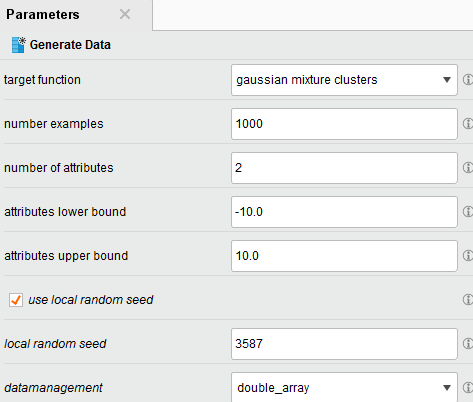
\includegraphics[width=0.4\linewidth]{figure/2-10}
\caption{\ 生成随机数据参数设置}
\label{fig:2-10}
\end{figure}


调用“Map”映射操作符,设置参数如图2-8,将所有的数据类型都转换为normal类型。

\begin{figure}[thbp!]
\centering
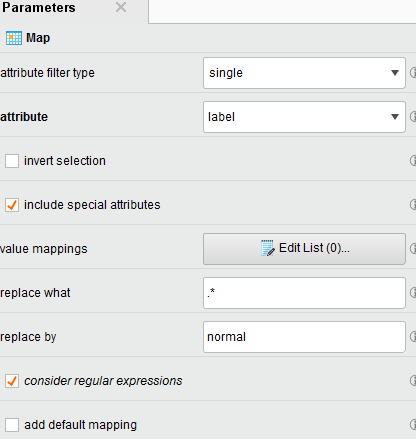
\includegraphics[width=0.4\linewidth]{figure/2-11}
\caption{\  映射操作符参数设置}
\label{fig:2-11}
\end{figure}


再次调用“Generate Data”生成数据操作符,参数设置如图2-9,添加离群点

\begin{figure}[thbp!]
\centering
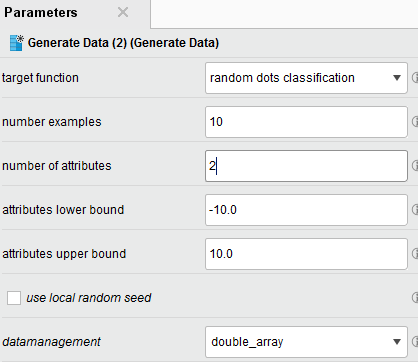
\includegraphics[width=0.4\linewidth]{figure/2-12}
\caption{\  添加离群点参数设置}
\label{fig:2-12}
\end{figure}


同样,添加Map操作符,参数设置如图2-10

\begin{figure}[thbp!]
\centering
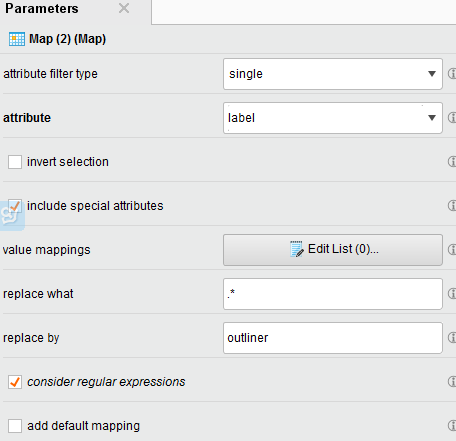
\includegraphics[width=0.4\linewidth]{figure/2-13}
\caption{\ Map映射离群点设置}
\label{fig:2-13}
\end{figure}


最后添加“Append”操作符将两个数据集合并,全部操作流程图如图2-11,数据散点图如图2-12.

\begin{figure}[thbp!]
\centering
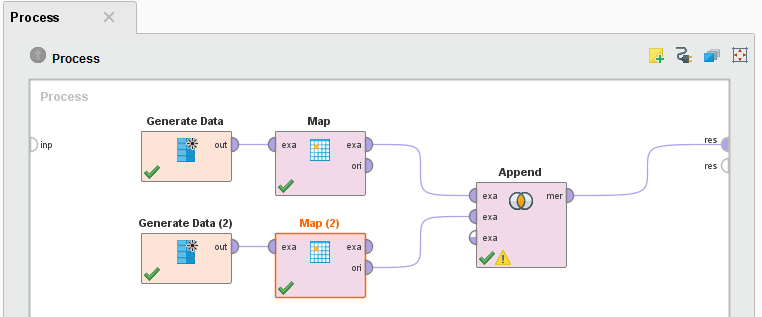
\includegraphics[width=0.4\linewidth]{figure/2-14}
\caption{\ 1.操作流程图}
\label{fig:2-14}
\end{figure}


\begin{figure}[thbp!]
\centering
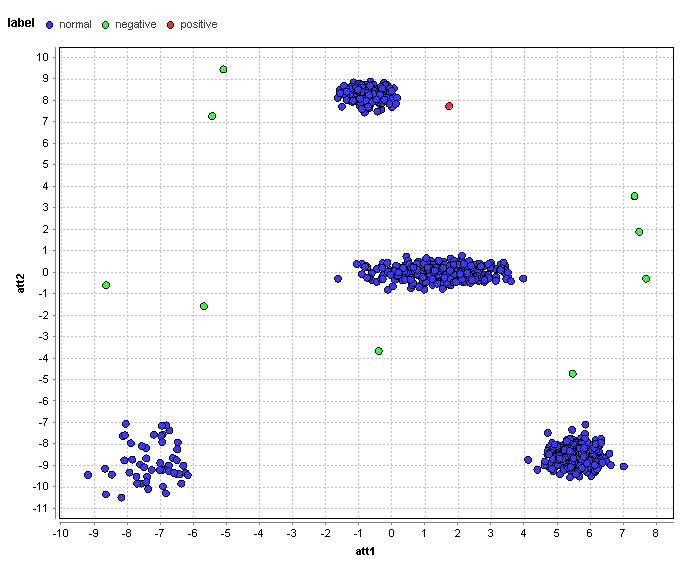
\includegraphics[width=0.4\linewidth]{figure/2-15}
\caption{\ 2.数据散点图}
\label{fig:2-15}
\end{figure}

第二步:离群点检测操作符应用

“k-NN Global Anomaly Score”k-NN全局离群点检测操作符,检测结果如图2-13

\begin{figure}[thbp!]
\centering
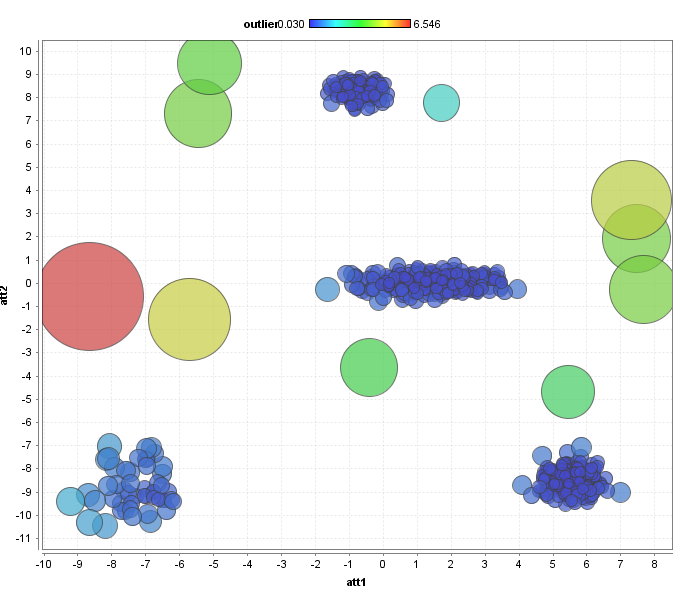
\includegraphics[width=0.4\linewidth]{figure/2-16}
\caption{\ 全局离群点检测气泡图}
\label{fig:2-16}
\end{figure}

“Local Outlier Factor”基于本地的离群点检测操作符,操作流程如图2-14,检测结果如图2-15

\begin{figure}[thbp!]
\centering
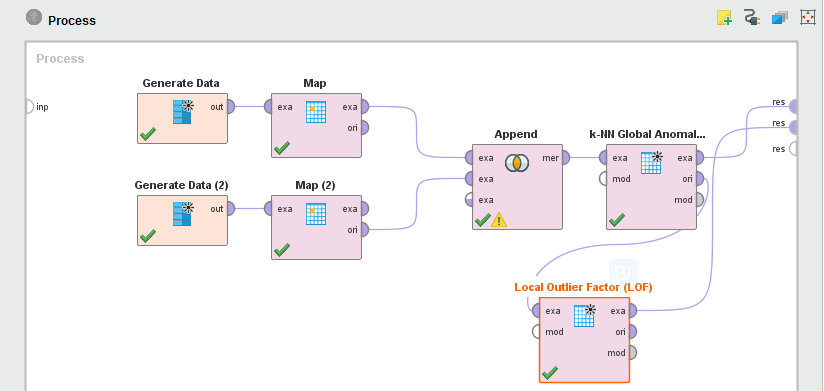
\includegraphics[width=0.4\linewidth]{figure/2-17}
\caption{\ 离群点检测操作流程}
\label{fig:2-17}
\end{figure}

\begin{figure}[thbp!]
\centering
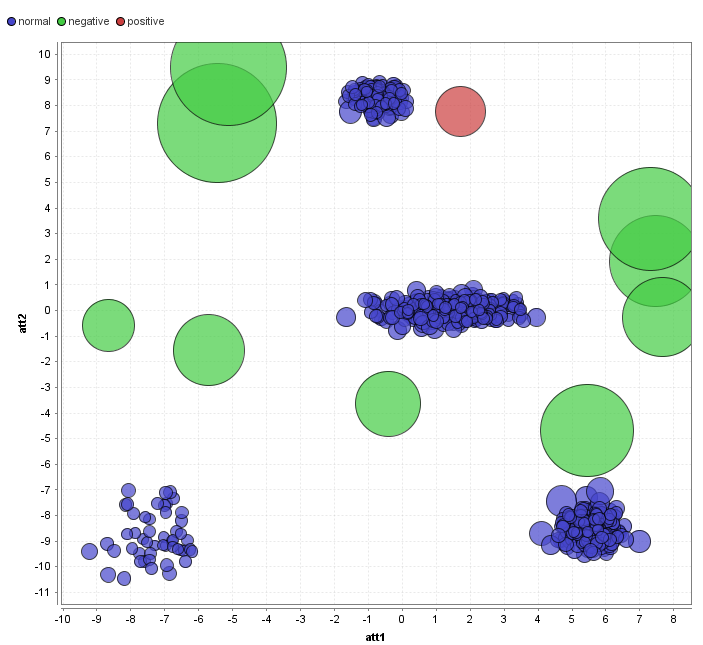
\includegraphics[width=0.4\linewidth]{figure/2-18}
\caption{\ 离群点检测操作流程}
\label{fig:2-18}
\end{figure}

